% TODO: Use twoside for printing
\documentclass[12pt]{report}
% English hyphenation, among other things
\usepackage[british]{babel}
% Use UTF-8 encoding
\usepackage[utf8]{inputenc}
% Better support for accented characters
\usepackage[T1]{fontenc}
% References
\usepackage{biblatex}
\addbibresource{references.bib}
% For quotes
\usepackage{csquotes}
% For cross references
\usepackage{hyperref}
% Graphics
\usepackage{graphicx}
\graphicspath{{images/}}
% A4 paper size with reasonable margins
% TODO: Modify bindingoffset for two-sided printing
\usepackage[a4paper,width=150mm,top=25mm,bottom=25mm,bindingoffset=6mm]{geometry}
% Fancy headers
\usepackage{fancyhdr}
% Make the headers fancy by default
% To clear headers, use \pagestyle{empty} followed by \pagestyle{fancy} to get the headers back
\pagestyle{fancy}
\setlength{\headheight}{15pt}
% Beautiful IBM Plex font families
%\usepackage{plex-serif}
\usepackage{plex-sans}
%\usepackage{plex-mono}
% Text coloring
\usepackage{color}
% Math blocks
\usepackage{amsmath}
% Math symbols
\usepackage{amssymb}
% Algorithms
\usepackage{algorithm}
\usepackage{algorithmicx}
\usepackage{algpseudocode}

\newcommand{\com}[1]{{\color{red}#1}} % supervisor comment

\begin{document}

\begin{titlepage}
    \sffamily
    \setlength{\parindent}{0pt}
    
\includegraphics[width=0.4\textwidth]{ntnu}

    \vspace*{2cm}

    \Huge
    \textbf{Top-k Spatial Join on GPU}

    \vspace{0.5cm}
    \LARGE
    % TODO: Remove this before submission
    % DRAFT, \today

    \vspace{1.5cm}

    \textbf{Erlend Åmdal}

    \vfill

    \large
    TDT4501 --- Computer Science, Specialization Project

    Fall 2019

    \vspace{1cm}

    Supervisor: Kjetil Nørvåg, IDI

    \vspace{1cm}
    Norwegian University of Science and Technology\\
    Department of Computer Science
\end{titlepage}

\chapter*{Abstract}
Given two sets of spatial objects \(R\) and \(S\) where each object is assigned a score, a spatial join predicate (such as a point distance threshold), and an aggregate function that combines scores for two objects (such as a simple sum), the top-k spatial join operation joins \(R\) and \(S\) by the spatial predicate and returns the \(k\) pairs with the best scores according to the aggregate function. The R-tree is a common spatial data structure that is a balanced search tree designed to accelerate spatial queries, which can be applied to evaluate spatial joins. Some methods have been proposed for the evaluation of top-k spatial joins, but they have not been explicitly designed for parallelism.

Graphics processors are becoming commodity hardware, and their massively parallel processing capabilities can be used to achieve high performance. APIs such as CUDA have enabled the trend of general-purpose computing on graphics processors (GPGPU), which has become a popular way to utilize this hardware. However, special application design is required to efficiently utilize GPGPU, which requires new research to adapt to the new computing paradigm. It has been shown that some spatial queries can be sped up significantly with GPGPU, but little research has been made into processing top-k spatial joins (and top-k queries in general) with graphics processors.

This thesis covers important aspects of processing top-k spatial joins using R-trees on GPU\@. Research suggests that some existing methods have potential to be adapted for GPGPU. We deal with some of the challenges that come with adapting applications for GPGPU. We define an R-tree memory layout designed for efficient random access in global memory, a bulk loading implementation based on GPU segmented radix sort and parallel reductions, and an adaptation of the Block-based algorithm for top-k spatial joins that utilizes varying degrees of parallelism.

\chapter*{Acknowledgements}
I wish to thank my supervisor Kjetil Nørvåg for this project proposition and for invaluable assistance in the writing of this thesis.

\tableofcontents
% Not particularly useful right now
% TODO: Add this
% \listoffigures

\chapter{Introduction}
In many applications, objects have both spatial attributes and non-spatial attributes. As an example, an application such as Google Maps provides points of interest and businesses, primarily with their geographic location, but also with reviews, user ratings and various other metadata. Spatial objects are also recorded in scientific fields such as atmospheric, oceanographic and environmental sciences with measurements of several attributes such as temperature, pressure and seismic activity.

Object attributes can be used as scores to derive a ranking, which often is used to perform a top-k query when the amount of objects is too large for all objects to be relevant. A top-k query retrieves the k objects with the best ranking. A top-k join is a special case of a top-k query which is performed on the results of a join. If the inputs of the join are each given a score, a top-k join can retrieve the top-k joined tuples that maximize an aggregate score, such as the average score.

A spatial join retrieves pairs of spatial objects that satisfy a spatial predicate, such as retrieving all intersecting pairs of objects or all pairs of objects within a certain distance from each other. As an example, given a set of all restaurants and a set of all hotels in Oslo, we would like to find pairs of restaurants and hotels that are within 1000 meters from each other for an overnight visit and dinner. The amount of restaurants and hotels within 1000 meters of each other will result in too many pairs to work with, so we would like to limit our search to highly rated pairs. We can make this top-k query, where we would like to find the 10 pairs of restaurants and hotels with the best total rating. Highly rated locations can easily be found, but the most highly rated locations are not necessarily found in close proximity to each other. We can find many pairs of locations that are close to each other, but we may not find the pairs with the best ratings quickly. An efficient solution must be able to use both their locations and their ratings to answer the query.

A spatial join can be an expensive operation because spatial datasets can be complex and very large. Spatial indexing data structures such as R-trees were created to increase the performance of spatial queries, and can be used to perform efficient spatial joins. By adapting methods from ranked joins, it is possible to answer top-k spatial joins even more efficiently by only evaluating the parts of spatial joins that are necessary to compute the answer. 

R-trees were traditionally designed to optimize I/O performance. With hardware trends such as reduced I/O costs, increasing memory sizes, multicore processors and graphics processors becoming commodity hardware, new methods are invented to fully utilize the hardware. One way to increase performance is by exploiting parallelism, which is enabled by multicore processors, distributed computing and graphics processors. However, traditional methods often require careful redesign to exploit parallelism, or entirely new methods must be designed.

The trend of General Purpose computing on Graphics processors (GPGPU) is enabled by programmable graphics processors using APIs such as CUDA\@. GPGPU presents an opportunity to achieve massively parallel computation, but not without limitations. The architecture of GPUs and CPUs are dissimilar in ways that require special application design to be able to fully utilize the resources of a GPU, and not all tasks are suited for GPGPU.\@ The use of GPGPU in certain database operators has been studied and has been shown to have speedups compared to CPU for operations such as relational joins~\cite{he2008relational} and spatial joins~\cite{yampaka2012spatial}. We would like to find out if similar speedups can be achieved for top-k spatial joins using GPGPU.\@

Top-k queries, top-k joins and spatial joins have been extensively studied. However, joins considering both spatial and score attributes at the same time have received limited attention~\cite{qi2013efficient}. 

\section{Related Work}

%\begin{figure}[h]
%    \centering
%    
\includegraphics[scale=0.5]{ntnu}
%    \caption{Norwegian Institute of Science and Technology}
%    \label{fig:ntnu}
%\end{figure}

\chapter{GPGPU}
General-purpose computing on graphics processors (GPGPU) is the use of a graphics processing unit (GPU) to perform computation that would traditionally be performed on the central processing unit (CPU). The majority of GPUs today are programmable using APIs such as OpenCL and CUDA.\@ Using these APIs, applications can utilize GPUs as coprocessors to execute parts of the application.

GPUs are particularly well-suited for problems that can be expressed as data-parallel computations, which is executing the same program on many data elements in parallel, ideally with high arithmetic intensity. Arithmetic intensity is the ratio of arithmetic operations to memory operations. Graphics processing is the original application, but GPUs have found widespread application in other areas such as machine learning.

This chapter focuses on the architecture of NVIDIA GPUs and the CUDA API.\@

\section{GPU architecture}

GPUs have some significant architectural differences to CPUs, something programmers must be aware of to fully utilize the capabilities of GPUs. The architecture of CPUs is designed for a variety of applications, while the architecture of GPUs is designed primarily for graphics applications. The main differences are that GPU memory is divided into multiple regions with different capacities, bandwidths, latencies and access methods, threads on a GPU can communicate in a number of specialized ways and branching instructions are carried out very differently from CPUs.

GPU architectures evolve over time, which exposes new features to programs and influences the way programs must be designed to optimally utilize the available resources. The features of the GPU architecture are expressed as the compute capability which is a string consisting of a major and minor version number, which at the time of writing ranges from 1.x to 7.x. This chapter describes devices with compute capability 6.x and 7.x, which is available in the most recent generations of hardware at the time of writing.

Unlike the CPU, the GPU dedicates most of its resources to data processing instead of caches and control flow mechanisms. Therefore, the cost of memory accesses and branching is high compared to the cost of data processing such as arithmetic operations. This means that programs with high arithmetic intensity are favored. The individual performance of each thread on a GPU is much lower than the performance of a thread on a CPU, but the GPU makes up for it with the sheer amount of threads that it can execute in parallel.

A GPU contains an array of Streaming Multiprocessors (SMs) and a large shared global memory. The multiprocessors can access the global memory and have an L2 cache that is shared by all multiprocessors. Each multiprocessor has its own L1 cache and on-chip memory that is only accessible to the multiprocessor. The GPU and CPU are connected through an interface such as PCI-e. The bandwidth of the global memory is much higher than the bandwidth between the GPU and CPU.\@ Similarly, the bandwidth of the on-chip memory is much higher than the bandwidth of the global memory.

Work is carried out by creating groups of threads to run a program, and distributing threads between the multiprocessors in groups of 32 parallel threads called warps. Groups of threads may be interdependent and must be scheduled onto the same multiprocessor. Each multiprocessor creates, manages, schedules and executes threads in warps. A warp is the smallest unit of threads, meaning that instantiating a number of threads that is not divisible into warps requires leaving the remainder of threads unutilized. All threads within a warp share a single program but have their own program counters and register states. Warps execute independently, but may share a program and shared memory with other warps in the same multiprocessor, and may also share the program and global memory with warps on other multiprocessors.

Within the multiprocessors, warps are executed with a Single Instruction, Multiple Thread (SIMT) architecture, meaning a warp executes one common instruction at a time on all 32 threads in parallel. Full efficiency is realized when all 32 threads have non-divergent execution paths. When the execution paths diverge, the warp can execute only one common instruction of a subgroup of threads at a time by disabling non-participating threads. Because warps execute independently, the effects of branch divergence only happen within a warp.

The execution of warps within a multiprocessor is efficiently interleaved by warp schedulers, so that an instruction can be executed while the results of other instructions still pending, even interleaving with instructions from other warps. Within a multiprocessor, a context switch from one warp to another has no cost. This is made possible by maintaining the program counters, registers and local memory used by a warp on-chip during the entire lifetime of the warp, even when other warps are executing. Each multiprocessor has a set of registers that are allocated between the warps. The amount of warps that can be executed concurrently by a multiprocessor therefore depends on the requirements of the warps.

Each multiprocessor has on-chip memory with higher bandwidth and much lower latency compared to that of global memory. The local memory is a sequence of 32-bit words distributed into 32 equally sized memory banks. Each memory bank has a bandwidth of 32 bits per clock cycle. A shared memory request for a warp allows each thread to access their own 32-bit word in a single clock cycle provided there is no bank conflict. A memory bank can broadcast a single 32-bit word to all threads requesting the same word, but concurrent access to multiple words within the same bank cannot be serviced in a single clock cycle, which generates a bank conflict. If a bank conflict occurs, the request is split into as many separate conflict-free requests as necessary.

Global memory is accessed via naturally aligned 32-, 64- or 128-byte memory transactions with an important feature called coalescence. When a warp executes an instruction to access global memory, it will attempt to coalesce the memory accesses into one or multiple memory transactions instead of performing a number of transactions per thread. Optimal throughput is generally achieved with the smallest amount of transactions with the least amount of unused words.

\section{CUDA}

CUDA distinguishes two entities, the host and the device. The host has the main memory and the CPU that runs the host program, while the device is a GPU serving as a coprocessor with its own memory. The host can allocate memory on the device and initiate memory transfers between main memory and device memory. The host can use the CUDA API to schedule programs to run on the GPU.\@

The most popular way to use CUDA is by extensions to C or C++ that allows writing programs with parts that run on the host and parts that run on the device. The parts of the program that run on the device are written using the same programming language syntax but use special annotations to utilize parts of the CUDA API, creating a low barrier of entry for C/C++ developers. Feature parity with C and C++ for code that runs on the device is mostly preserved, but there are some notable documented exceptions to which features are available.

The unit of execution in CUDA is a kernel instance. A kernel is a function that can be executed \(N\) times in parallel by \(N\) different CUDA threads by instantiation. When a kernel is instantiated, the caller must specify a number of thread blocks and the number of thread per block that will be used to carry out the execution. The division into thread blocks forms the boundaries for thread cooperation. Each thread block is an independent part of the execution of the kernel, while the threads within each thread block can cooperate.

Threads within the same thread block can cooperate efficiently using a number of mechanisms. Threads can exchange data using memory that is shared by all threads in a group or use barriers and memory fences to synchronize their execution. Because threads are executed in warps, there are also special synchronization mechanisms that allow exchanging data within warps.

Threads and thread blocks are composed into grids. A kernel instance has a grid of thread blocks, and each thread block has a grid of threads. Grids are three-dimensional, but not all dimensions of the grid have to be used, so each element in a grid can be identified using a one-dimensional, two-dimensional or three-dimensional index. The thread index and group index can be used by threads to assign each thread to an individual element in a domain such as a vector, matrix, or volume.

Memory in CUDA is divided into a hierarchy. Each CUDA thread has its own private memory, each thread group has its own shared memory, and all threads have a shared global memory. Global memory is memory that can be accessed both by the host and the kernels. It is the memory with the greatest capacity, typically measured in gigabytes, but is also the memory with the greatest access cost. The host program can freely dynamically allocate global memory, though kernels can do it only to a lesser extent. Shared memory is local to each thread group. It has much lower access cost than global memory, but its capacity is limited by the on-chip memory, commonly between only 48 KB and 92 KB. Shared memory is not dynamically allocated, it is instead statically allocated for each thread group. Private memory has the lowest potential access cost and is also statically allocated. It is primarily stored in registers and is therefore the fastest, but may have to be stored in local memory, which is actually thread-local global memory. Shared memory is stored in the on-chip memory banks. Global memory is stored on the device and is cached by L1 and L2 caches.

Thread blocks are required to execute independently. Thread blocks can be executed in any order, both in parallel and in series. This means that cooperation between thread blocks is not allowed. This programming limitation is key to allow flexibility for the device to find the optimal execution plan to schedule thread blocks across multiprocessors based on its architecture and available resources.

All threads in a thread block are scheduled onto the same multiprocessor. The threads are divided into \(\lceil\frac{T}{W_{size}}\rceil\) warps where \(T\) is the number of threads per block and \(W_{size}\) is the warp size, equal to 32. All warps in a thread block are scheduled onto the same multiprocessor. The execution of each warp is independent and interleaved. If the execution of a warp does not depend on the execution of other warps, it does not have to explicitly synchronize with other warps from the same thread group. Otherwise, memory fences and barriers can be used to synchronize across across warps.

CUDA is an asynchronous API, meaning that the execution on the host and the device may happen asynchronously. The host can schedule tasks such as memory transfers and kernel calls into sequences called streams. Tasks may be executed concurrently and out of order unless the tasks are scheduled in order into the same stream. The host can explicitly synchronize with a stream, for instance to read the result of a kernel execution.

\section{Performance optimization}

The performance of a CUDA application can scale with hardware advancements in multiple ways. The addition of more multiprocessors can increase performance, provided the application can efficiently utilize all multiprocessors, usually by scheduling a sufficient amount of thread blocks. New features added with increased compute capability can be utilized. The clock speed, instruction speed and memory sizes and bandwidths can all be increased. CUDA allows programs to be compiled into an intermediary executable format that allows the hardware and driver to optimize for its architectural features.

A program that parallelizes over a set of threads with little cooperation between threads should generally prefer dividing the set of threads into as many independent thread groups as possible while respecting the warp size.

Programs should utilize local memory for frequently accessed data that is shared by threads in thread groups, with access patterns that avoid bank conflicts.

Requests to global memory should optimize for coalescence. This is achieved by making requests to dense areas of memory and aligning them with naturally aligned 32-, 64- and 128-bit transactions.


\chapter{Spatial indexing}
The goal of indexing is to improve the efficiency of searches. For spatial indexing, the goal is to improve the efficiency of processing spatial queries. Spatial queries relate to the attributes of spatial objects such as their positions and sizes and whether or not they intersect with each other. This can be achieved with spatial data structures such as the R-tree.

\section{Concepts}

A spatial object can be a point, a line, a polygon, or any other shape in the real coordinate space of \(d\) dimensions \(\mathbb{R}^d\). Using set theory, a spatial object in \(\mathbb{R}^d\) can be considered a potentially infinite set of points \(X\) such that \(X \subseteq \mathbb{R}^d\).

Set operations have geometric interpretations. As an example, given two spatial objects \(X\) and \(Y\), \(X \cap Y\) is a spatial object consisting of the space covered by both objects, which is the intersection of the two objects.

A spatial predicate is a relation between spatial objects. For instance, given spatial objects \(U\) and \(V\), \(U\) and \(V\) are said to intersect if \(U \cap V \neq \emptyset\), and \(U\) is said to contain \(V\) if \(U \supseteq V\). Spatial predicates may have properties that are useful for processing spatial queries. For instance, any object that contains an object \(U\) that intersects with an object \(V\) must also intersect with \(V\).

A point \(p\) in \(d\)-dimensional space can be represented as a \(d\)-dimensional vector \((p^{[1]}, p^{[2]}, \dotsc, p^{[d]})\) where \(p^{[i]}\) denotes the \(i^{th}\) coordinate of \(p\). A point may be a spatial object in the form of a singleton, which is a set with exactly one element, the point itself.

An axis aligned box is a spatial object in the form of a box where the edges of the box are parallel to the coordinate axes. An axis aligned box is defined by two points \(B = (b, t)\) where
\[
  \forall i \in \{1, \dotsc, d\} :
  b^{[i]} \leq t^{[i]}
\]
where \(p^{[i]}\) denotes the \(i^{th}\) coordinate of the point \(p\). \(b\) can be considered the \emph{bottom point} and \(t\) can be considered the \emph{top point}. The axis aligned box contains points so that for each dimension \(i\), \(b^{[i]}\) is the minimum (bottom) coordinate and \(t^{[i]}\) is the maximum (top) coordinate. That is,
\[
  B = \{
    q \in \mathbb{R}^d \mid
    \forall i \in \{ 1, \dotsc, d \} :
    b^{[i]} \leq q^{[i]} \leq t^{[i]}
  \}
\]

The axis aligned Minimum Bounding Box (MBB) of a spatial object \(X\) is the axis aligned box with the smallest measure that covers \(X\). Depending on the dimensionality of the space, the measure of a spatial object can be the length, area, volume or hypervolume of the object. Axis aligned MBBs are commonly used to approximate the locations of spatial objects and can be used as a simple descriptor of the shape of a more complex spatial object.

It follows that that \(X \subseteq \textrm{MBB}(X)\), which implies that any spatial object that intersects with \(X\) must also intersect with \(\textrm{MBB}(X)\). For complex geometry, this has practical applications to speed up computations for spatial operations.

The axis aligned MBB of a spatial object \(X\) can be represented as \(B = (b, t)\) where
\[
  \forall i \in \{ 1, \dotsc, d \} :
  b^{[i]} = \min\left( q^{[i]} \mid q \in X \right)
  ,
  t^{[i]} = \max\left( q^{[i]} \mid q \in X \right).
\]

\section{Spatial join queries}

The spatial distance join returns pairs of objects that are close to each other. More formally, given two sets of spatial objects \(R\) and \(S\), a distance metric dist and a distance threshold \(\epsilon\), the spatial distance join returns
\[
  \{ (r, s) \in R \times S \mid \mathrm{dist}(r, s) \leq \epsilon \}.
\]

\(dist\) is defined to return the distance between the points of the two spatial objects that are closest to each other according to a distance function \(p\).

\[
  dist(r, s) = \min\left(p(t, u) \mid t, u \in r \times s \right)
\]

For instance, \(p\) could be the Euclidean distance, which is the straight-line distance between two vectors. We can also use the Chebyshev distance, where the distance is the greatest of the differences along any coordinate dimension.

\(dist(r, s) \leq \epsilon\) is a type of spatial predicate. For \(\epsilon = 0\) it is equivalent to intersection. Using the Chebyshev distance measure between two bounding boxes \(r\) and \(s\), we can think of it as expanding either \(r\) or \(s\) by \(\epsilon\) and testing for intersection.

For the purposes of spatial indexing, the distance metric will primarily operate on points and axis aligned boxes. This simplifies finding the pair of points that are closest to each other according to the distance function. For pairs of spatial objects that are points, the distance function is simply computed directly on the points. For pairs of spatial objects that are axis aligned boxes, the closest points can be found on the box boundaries, unless the boxes intersect, in which case the distance is zero.

\section{R-trees}

The R-tree~\cite{guttman1984r} can be considered a multidimensional version of the B-tree, which is a balanced search tree. The keys of the R-tree are axis aligned boxes which can be spatially queried. It is commonly used as an indexing structure for spatial queries.

Conceptually, the R-tree partitions the key space into a hierarchy of MBBs where key boxes are placed at the bottom. Each MBB in the hierarchy consists of the MBB of its children. MBBs at the same level in the hierarchy may overlap with each other.

The R-tree is a balanced tree structure consisting of a number of nodes divided into levels. Nodes in all levels but the lowest level are inner nodes, while nodes at the lowest level are leaf nodes. Entries are placed in the leaf nodes, each containing a link to a data object along with the key box. Inner nodes contain similar entries, except they link to lower level nodes instead of data objects along with the MBB of the lower level node. A leaf node is said to contain a data object if any of its entries point to the data object. Similarly, an inner node is said to contain a data object if any of its ancestor leaf nodes contain the data object. In figure \ref{fig:r-tree}, A is the root node, which is an inner node. B, C and D are leaf nodes which are entries of the root node. E, F, G, H, I and J are leaf node entries.

\begin{figure}[h]
    \centering
    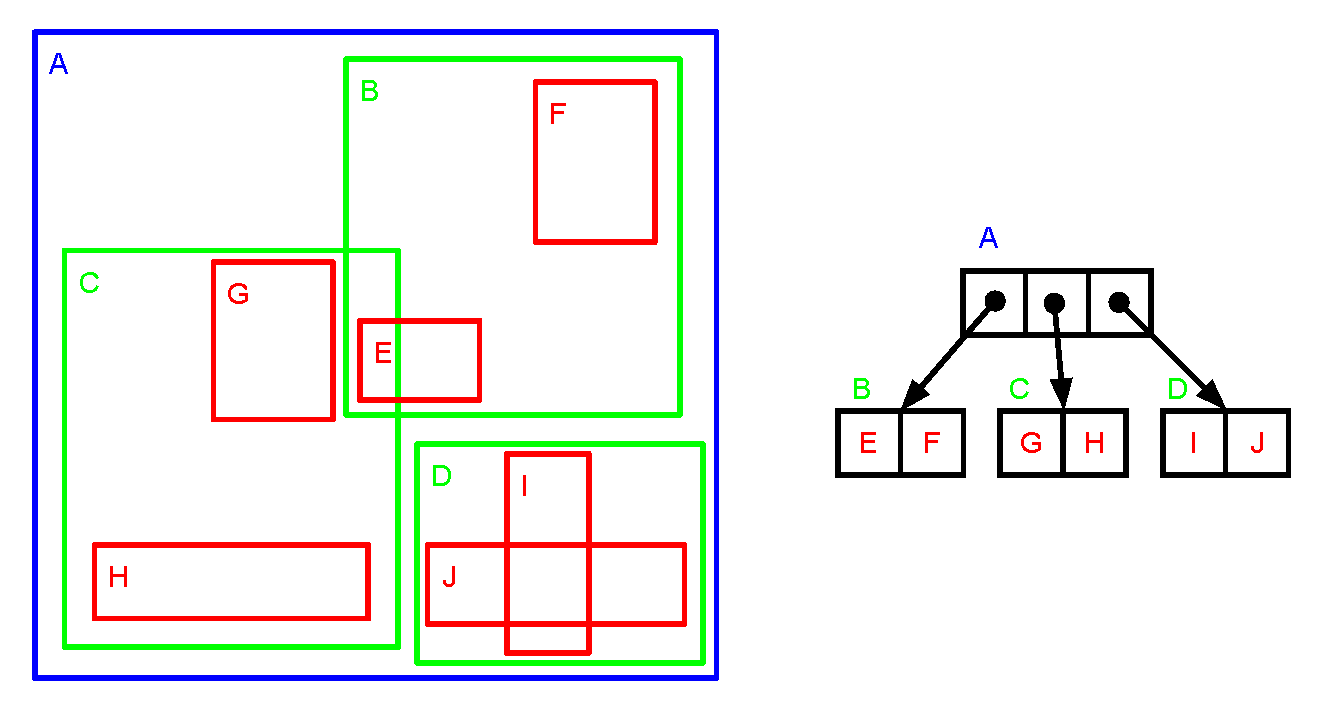
\includegraphics[scale=0.5]{r_tree}
    \caption{R-tree}
    \label{fig:r-tree}
\end{figure}

Values are inserted as entries in leaf nodes. To keep the tree balanced and to avoid nodes growing too large, all nodes but the root node must have between \(m\) and \(r\) entries where \(m \leq \frac{r}{2}\). \(r\) is the maximum amount of entries in an R-tree node, and is called the \emph{fanout}. The root node can have anywhere from \(0\) to \(r\) entries. If inserting an entry into a leaf node would result in more than \(r\) entries, the node has to be split into two leaf nodes by creating a new leaf node and partitioning the entries between them. The newly created leaf node has to be inserted into the parent node, which may result in the parent node requiring a similar split. The split can propagate up to the root, in which case the root also must be split, and another level has to be added to the tree.

The query performance of an R-tree is a measure of the average amount of nodes that have to be visited to perform a search. When searching, it is desirable to visit as few nodes as possible, as each branch of each node has to be evaluated, and accessing a node may have a cost (depending on the memory layout). For good query performance, R-tree nodes should be packed as fully as possible, and branches should have minimal overlap. Packed nodes decrease the height of the tree, which reduces the amount of nodes that have to be accessed to reach the leaves. When the cost of accessing a node outweighs the cost of evaluating branches, packed nodes reduce the total amount of nodes which results in fewer nodes that have to be accessed to perform a search. Minimal overlap between branches allows the search to more easily narrow down to fewer subtrees.

The R-tree has been extensively researched and used, and has inspired the creation of variations such as the R*-tree~\cite{beckmann1990r}, the R+-tree and the revised R-tree. Most of the variations preserve the data structure and principles while redefining the insert and remove operations. Operations that modify the tree can be designed for varying degrees of query performance at the cost of the performance and complexity of operations to insert and delete values.

\subsection{aR-trees}

The aR-tree is an R-tree that has been augmented with aggregate values assigned to each node. Similar to how the MBB of a node is an aggregation of the boxes of all objects placed under it, other types of object attributes can be aggregated to enhance the search capabilities of the tree. An example aR-tree is the IR-tree~\cite{li2010ir} which is augmented for spatio-textual searches by storing aggregated inverted files in each node. A simpler example is an aR-tree that stores the maximum and minimum value of an attribute for all objects under the node, which may have practical applications in databases.

The aggregated attribute of an aR-tree node \(N.agg\) is defined by a value function \(v\) and a decomposable aggregate function \(\gamma\). \(v\) retrieves values from object that can be aggregated by \(\gamma\). For leaf nodes, the aggregate value is computed directly as the aggregation of \(v\) for all objects contained by the leaf node. For inner nodes, the aggregate value is computed as the aggregation of the \(N.agg\) values of its child nodes. It follows that the aggregate value of any node is the aggregation of \(v\) for all R-tree entries under the node.

The aggregate values stored in the aR-tree augment the search capabilities of the R-tree because each inner node carries information that can be used to assert certain properties about contained values. By using the MAX aggregate function on \(v(O)\) when searching for objects with the condition \(v(O) \geq v_{\min}\), it can be asserted that only inner nodes with \(N.agg \geq v_{\min}\) can contain values satisfying the condition. The MAX aggregate function also guarantees that the entry with the greatest \(v(O)\) can be found by descending the tree and always choosing the inner node with the greatest aggregate value.

\begin{figure}[h]
    \centering
    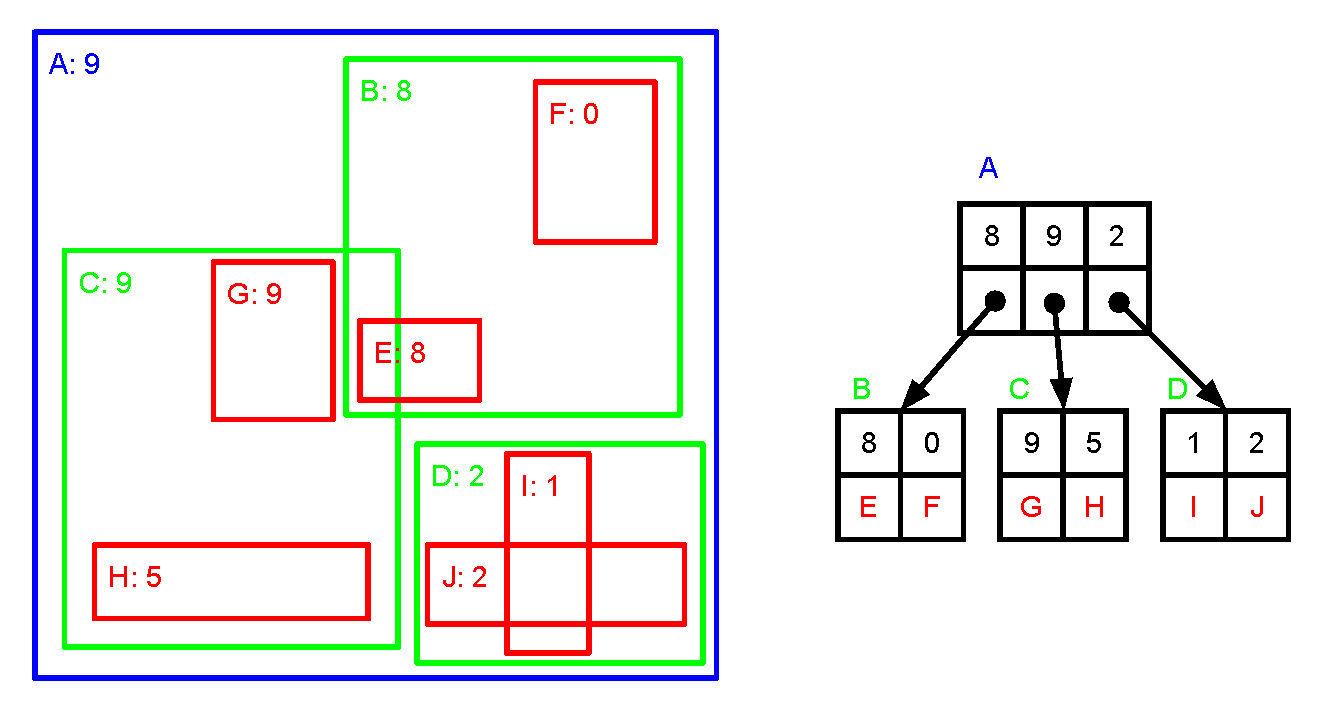
\includegraphics[scale=0.5]{max_ar_tree}
    \caption{MAX aR-tree}
    \label{fig:max-ar-tree}
\end{figure}

% Operations that modify aR-trees require updating the aggregate values. When an entry with aggregate value \(s\) is added to a node \(N\), either as \(s = v(O)\) for an object \(O\) or as \(s = M.agg\) for a node \(M\), the aggregate value of \(N\) can be updated as \(N.agg' = \gamma(N.agg, s)\). When an entry is removed from a node, the aggregate value of the node has to be recomputed from the remaining entries.

\subsection{Range search using R-trees}

A range search on an R-tree returns the leaf entries whose MBBs intersect with the query box. Algorithm~\ref{alg/r-tree-range-search} can be described as an iterative operation on a LIFO (Last-In-First-Out) queue. The queue is initialized with the entries of the root node. Entries are dequeued until the queue is empty. If the dequeued entry is a leaf node entry, it is made part of the result. If the entry is an inner node entry, all its children are enqueued. A query box that does not intersect with the MBB of a node \(N\) cannot intersect with any objects contained by \(N\). Therefore, a non-intersecting node and all its ancestors can be pruned from the search because they will not output any results.

\begin{algorithm}
  \caption{R-tree Range Search. \(N\) is any R-tree node, but usually the root node of the R-tree. \(Q\) is the query box.}
  \label{alg/r-tree-range-search}
  \begin{algorithmic}[1]
    \Function{RangeSearch}{\protect\(N, Q\protect\)}
      \State \(O \leftarrow \emptyset\)
      \State Initialize \(Queue\) as a queue with entries of \(N\).
      \While{\(Queue\) is not empty}
        \State \(E \leftarrow\) \Call{Dequeue}{\protect\(Queue\protect\)}
        \If{\Call{Intersects}{\protect\(E.mbb, Q\protect\)}}
          \If{\(E\) is a leaf entry}
            \State \(O \leftarrow O + E\)
          \Else
            \ForAll{\(C \in E.ref\)}
              \State \Call{Enqueue}{\protect\(Queue, C\protect\)}
            \EndFor
          \EndIf
        \EndIf
      \EndWhile
      \State \Return \(O\)
    \EndFunction
  \end{algorithmic}
\end{algorithm}

While range search concerns spatial intersection with a query box, it is possible to generalize for other predicates provided they have a similar property. The specific property required of a predicate \(\phi\) is as follows,
\[
  \forall A, A' \in \mathbb{P}(\mathbb{R}^d) : (A \subseteq A') \wedge \phi(A) \Rightarrow \phi(A')
\]
where \(\mathbb{P}(\mathbb{R}^d)\) is the set of all spatial objects in the \(d\)-dimensional space \(\mathbb{R}^d\). An interpretation is that a if the predicate is true for a spatial object \(A\), it must also be true for any larger object that contains \(A\). In the case of an R-tree range query, \(\phi\) tests for intersection with a query box, where \(A\) is a box of a leaf node entry and \(A'\) is the MBB of any node that contains it. If an entry in an R-tree intersects with the query box, any node that contains the entry must also intersect with the query box, otherwise it would be pruned during the range search.

\subsection{Spatial join using R-trees}

R-trees can naturally be used to enhance the performance of spatial joins. As opposed to performing a nested loop join to test the spatial predicate for all pairs, R-trees can utilize the spatial characteristics of the inputs to reduce the amount of spatial predicate evaluations necessary to produce the output. R-trees can be built dynamically similarly to hash tables for relational joins, or they can be joined directly.

Brinkhoff et al.~\cite{brinkhoff1993efficient} described a method to concurrently descend down two R-trees to perform a spatial intersection join as described in algorithm \ref{alg-r-tree-spatial-intersection-join}. The algorithm is quite similar to the range search algorithm, except it searches for leaf entry tuples instead of individual leaf entries. Similar to the pruning in the range search algorithm, the spatial intersection join is based on the idea that if the MBBs of nodes \(N_R\) and \(N_S\) do not intersect, the objects they contain cannot form pairs \((key_R, key_S)\) where \(key_R\) and \(key_S\) intersect. Given well constructed R-trees, this allows pruning potential intersecting candidates at directory levels.

\begin{algorithm}
  \caption{R-tree Spatial Intersection Join. \(N_R\) and \(N_S\) are R-tree nodes from R-trees \(R\) and \(S\), usually the root nodes of their respective R-trees.}
  \label{alg-r-tree-spatial-intersection-join}
  \begin{algorithmic}[1]
    \Function{SpatialJoin}{\protect\(N_R,N_S\protect\)}
      \Comment{\(N_R\) and \(N_s\) must be at the same level}
      \State \(O \leftarrow \emptyset\)
      \State Initialize \(Queue\) as a queue with entry pairs of \(N_R \times N_S\).
      \While{\(Queue\) is not empty}
        \State \((E_R, E_S) \leftarrow\) \Call{Dequeue}{\protect\(Queue\protect\)}
        \If{\Call{Intersects}{\protect\(E_R.mbb, E_S.mbb\protect\)}}
          \If{\(E\) is a leaf entry}
            \Comment{\(S\) is also a leaf}
            \State \(O \leftarrow O + (E_R, E_S)\)
          \Else
            \ForAll{\(C_R \in E_R.ref\)}
              \ForAll{\(C_S \in E_S.ref\)}
                \State \Call{Enqueue}{\protect\(Queue, (C_R, C_S)\protect\)}
              \EndFor
            \EndFor
          \EndIf
        \EndIf
      \EndWhile
      \State \Return \(O\)
    \EndFunction
  \end{algorithmic}
\end{algorithm}

Like the range query, the algorithm can be described as an iterative operation on a LIFO (Last-In-First-Out) queue. The queue is initialized with all root node entry combinations. Tuples of branches are dequeued until the queue is empty. If the dequeued entries are leaf node entries, they are made part of the result. If the entries are inner node entries, all combinations of children entries are enqueued. A pair of nodes that do not intersect cannot contain intersecting entries. Therefore, tuples of non-intersecting nodes and all their ancestor tuples can be pruned from the search because they will not output any results.

For R-trees with different height, a more complete solution is required. In the case where \(S\) is taller than \(R\), the SpatialJoin algorithm will output entries \((E_R, E_S)\) where \(E_R\) is a leaf node entry in \(R\) while \(E_S\) is an inner node entry in \(S\) instead. In order to produce the expected spatial join outputs, for each output of SpatialJoin, a range search must be performed on the node referenced by \(E_S\) using \(E_R\mathrm{.mbb}\) as the query box. The output of the range search on \(E_S\) can then be output as tuples with \(E_R\).

While Brinkhoff et al.\@ only considered spatial intersection, it is possible to generalize for other spatial predicates provided they have a similar property. The specific property required of a spatial predicate \(\phi\) is as follows,
\[
  \forall A, A', B, B' \in \mathbb{P}(\mathbb{R}^d) : (A \subseteq A') \wedge (B \subseteq B') \wedge \phi(A, B) \Rightarrow \phi(A', B')
\]
where \(\mathbb{P}(\mathbb{R}^d)\) is the set of all spatial objects in the \(d\)-dimensional space \(\mathbb{R}^d\). An interpretation is that if the predicate is true for a pair of spatial objects \(A\) and \(B\), it must also be true for any pair of larger objects that contain \(A\) and \(B\). In the case of an R-tree join, \(A\) and \(B\) are boxes of leaf node entries from their respective R-trees, and \(A'\) and \(B'\) are the MBBs of nodes containing them. If entries of two R-trees intersect with each other, any node that contains the entries from each tree must also intersect with each other, otherwise they would be pruned during the range search.

The generalization of spatial predicates for range search and spatial joins is a necessary insight to apply the algorithms for other predicates than intersection. The property is intuitively true for the intersection predicate. The spatial distance threshold predicate can be considered equivalent to intersection where either object is \emph{expanded} by \(\epsilon\), therefore the property intuitively holds true for the spatial distance predicate.

\subsection{Search types and iterators}

Queues can be implemented in various ways for range searches with R-trees to create different kinds of searches. By replacing the LIFO queue with a FIFO queue, the search becomes a breadth-first search (BFS) instead of a depth-first search (DFS). When the order of the output matters, the queue can also be replaced by a priority queue to perform a best-first search, which has applications for ranked queries. aR-trees can provide necessary attributes to sort entries of inner nodes in the priority queue. Because the R-tree join is also based on a queue, similar results can be achieved.

A depth-first-search can be performed using a compact tree search iterator such as the one described in algorithm~\ref{alg-tree-search-iterator} instead of using an explicit queue. The iterator operates on a stack of node entry iterators. The stack will contain at most an iterator per level of the R-tree, and therefore has a fixed capacity equal to the height of the R-tree. The node entry iterator may simply be based on a pointer to an R-tree node and a number that counts the number of entries of the node that have been visited. The tree search iterator can also be applied to spatial joins by replacing the node entry iterator with an iterator that joins the entries of two nodes.

\begin{algorithm}
  \caption{DFS Tree Search Iterator. \(S\) is a stack of node entry iterators, initialized with a node entry iterator of the root node. \(\phi\) is the search predicate used to prune R-tree entries.}
  \label{alg-tree-search-iterator}
  \begin{algorithmic}[1]
    \Function{Next}{\protect\(S, \phi\protect\)}
      \While{\(S\) is not empty}
        \State \(I \leftarrow\) \Call{Peek}{\protect\(S\protect\)}
        \State \(E \leftarrow\) \Call{Next}{\protect\(I, \phi\protect\)}
        \If{\(E\) is Nil}
          \State \Call{Pop}{\protect\(S\protect\)}
        \Else
          \If{\(E\) is inner node entry}
            \State \(I_C \leftarrow\) \Call{NodeEntryIterator}{\protect\(E\protect\)}
            \State \Call{Push}{\protect\(S, I_C\protect\)}
          \Else
            \State \Return \(E\)
          \EndIf
        \EndIf
      \EndWhile
      \State \Return Nil
    \EndFunction
  \end{algorithmic}
\end{algorithm}

An explicit queue based search allows for parallel processing of queue elements by having multiple threads dequeuing and enqueuing elements in the same queue. This method can achieve data parallelism by both evaluating spatial predicates and traversing subtrees in parallel, but requires efficient synchronization mechanisms for the queue. The efficiency of this method depends on the amount of elements that can be processed in parallel, which may be limited by the amount of queue elements produced at each level in the search. For a narrow range search in a well constructed R-tree, the number of subtrees that must be visited should be low, which results in an overall small queue until the last few levels. Therefore, the gains for range queries would primarily be in parallel evaluation of spatial predicates. However, the queue is expected to grow exponentially for an R-tree spatial join, which suggests that parallel evaluation of spatial joins can be limited by the amount threads available rather than the size of the queue.

One way to utilize parallel processing of queue elements in range search is processing multiple range queries in parallel using the same queue. You et al.~\cite{you2013parallel} proposed and evaluated multiple methods to perform parallel range queries using GPUs.\@ Given an R-tree and a set of range queries to be performed on the R-tree, the algorithms efficiently computes the result of all range queries in parallel. It can be done by implementing existing methods for depth-first and breadth-first search for R-tree range queries on the GPU.\@

In the DFS method, each thread processes one query in depth-first order using a DFS tree search iterator. The main advantage of DFS is its predictable memory usage and simplicity. Each query requires only a stack with capacity equal to the height of the tree to perform the traversal, which can be stored in shared memory. The implementation is based on a count-and-write strategy that spaces out the memory prior to writing the query results. An issue with the DFS method is that it provides poor workload balance when queries require different amounts of work, leaving some threads idle and waiting for others to finish. The count-and-write strategy effectively requires evaluating all queries twice, which is speculated to harm performance. For particularly large queries, the writing of results to global memory may also be too sparse to coalesce.

The BFS method distributes the queries across multiple thread groups where each thread group has a queue in shared memory and all its threads working on the queue in parallel. Each queue entry is a \((N, Q)\) tuple where \(N\) is a pointer to an R-tree node and \(Q\) identifies a query. A queue entry \((N, Q)\) is expanded by dequeuing then enqueueing the children of N as \((N_C, Q)\) tuples, but only if the MBB of \(N\) and the query box of \(Q\) intersect. When a queue contains only leaf nodes, it is copied to global GPU memory to be made part of the result. Compared to the DFS method, the BFS method solves the workload balance problem within each thread group and has superior performance overall, but is more complex due to the limited capacity of the queue.

As previously stated, each queue in the BFS method has a fixed capacity imposed by the limited amount of shared memory that is available to each thread group. In a breadth-first search, the queue is expected to grow larger as the search goes deeper and may cause the queue to overflow. Calculating a distribution of queries that avoids overflow is infeasible, therefore the algorithm is designed to handle overflows. There are multiple alternatives for overflow handling strategies, and the most promising alternative dynamically allocates chunks of global memory for overflowing queues.

Performing a set of range queries on an R-tree is equivalent to performing an R-tree join using an R-tree constructed from the set of range queries. Given that range queries can be performed in parallel using the DFS and BFS methods, spatial joins could also be performed in parallel by modeling the problem as a set of range queries on an R-tree, but it would lack the main strength of the R-tree join algorithm, which is its ability to prune subtrees of both R-trees.

Given the queue-based search nature of DFS, BFS and the R-tree spatial join algorithm, it may be possible to adapt the DFS and BFS methods to perform parallel spatial joins, but some differences must be tackled. By considering each element of the queue as an independent task that either produces subtasks or outputs values, execution of parallel range queries starts with a large queue and therefore a large set of independent tasks that can easily be distributed in DFS and BFS. A spatial join, however, starts with a single queue entry and therefore only a single task. To efficiently perform a spatial join as independent tasks, the initial task must first be broken down into independent tasks.

\subsection{Memory layout}

Being originally designed for disk storage, the original R-tree uses a page-based layout. Nodes correspond to disk pages if the structure is disk resident, and memory pages otherwise. An R-tree node with this layout can contain as many entries as the page can fit as records. A notable feature is that the MBB of an R-tree node is stored along with the pointer to the node's page in an inner node record instead of being stored within the node's own page. This allows pruning the node without having to load the page. Loading a disk resident page has a significant I/O cost, but a memory resident page may also have an access cost because the page may have to be loaded into processor cache. The main advantage of the page-based layout is that modifying the structure of the R-tree only requires allocating and freeing pages and updating pointers to pages.

A page based layout would be inefficient on GPU. One difficulty with using the page-based layout on GPUs is transferring R-trees between main memory and device memory. Every source page would have to be replicated in the other memory by allocating a destination page and performing a memory transfer between the source and the destination per page. Destination pages may receive different memory addresses in the destination memory, requiring pointers to be updated. Additionally, R-trees with read-only usage would not benefit from strength of the page-based layout, which is its performance for operations that modify the structure of the R-tree.

Luo et al.~\cite{luo2012parallel} used two arrays to store the R-tree structure on a GPU.\@ The first is an array of integers representing the tree structure which is called \emph{Index}, and the second is an array of boxes called \emph{Rect}. For an R-tree with \(N\) nodes and a fanout of \(r\), both arrays consist of \(N\) blocks of \(r\) values. The root node is stored in the first block of both arrays. For inner nodes, each integer in a block of \emph{Index} is the array index of a child node, and each box in a block of \emph{Rect} is the MBB of the child node. For leaf nodes, each integer in a block of \emph{Index} is an identifier of an entry in the R-tree, and each box in a block of \emph{Rect} is the box of the entry. Non-full nodes are padded by zeroes in \emph{Index}.

The linearized R-tree memory layout used by You et al.~\cite{you2013parallel} stores the entire R-tree in an array of all nodes in breadth-first order. Inner nodes are represented by \(\{MBB, pos, len\}\) tuples, where \(MBB\) is the minimum bounding box of the node, \(pos\) is the position of the first child node in the array, and \(len\) is the amount of children. Because sibling nodes are stored sequentially in BFS order, their positions can be calculated by offsetting from the position of the first child. The specific layout of leaf nodes was left unspecified. The linearized R-tree memory layout is more compact than the layout used by Luo et al.~because inner nodes do not store a position per child, and there is no wasted memory for nodes that are not filled to capacity.

The linearized R-tree memory layout is optimized for read operations and memory transfers without serialization. It is designed to be cache friendly with its compact layout and sequential sibling node storage. The entire R-tree can easily be streamed between main memory and GPU memory by only streaming the the array. It should only be used for read-only R-trees. Write operations would require shifting nodes around in the array and recalculating pointers to child nodes to preserve DFS order and thus would perform poorly. Linearized R-trees can really only be constructed when the node layout is known in advance. Bulk loading methods may be adapted to construct linearized R-trees, or alternatively, a linearized R-tree may be constructed as a copy of another R-tree.

\subsection{Bulk loading}

R-tree bulk loading is the process of constructing an R-tree from an unindexed set of entries. When querying a set of unindexed entries, it may be beneficial to bulk load an R-tree prior to performing the queries, but bulk loading can be a costly operation. Prior bulk loading may enhance the performance of queries on unindexed sets, but only if the cost of performing unindexed queries outweighs the cost of bulk loading the R-tree and performing indexed queries. The choice of bulk loading strategy strongly affects the query performance. Bulk loading strategies often produce packed R-trees, which generally increases the query performance and reduces the memory usage of the R-tree.

Dynamic bulk loading is the most basic form of bulk loading where the R-tree is constructed by inserting one entry at a time. It is inherently sequential and relies on the efficiency of the insertion algorithm. A slow insertion algorithm may produce an R-tree with good query performance, but makes for a slow bulk loading strategy. A cheap insertion algorithm may make a faster bulk loading strategy, but the query performance of the resulting R-tree will suffer. Dynamic insertion also relies on dynamic allocation of nodes, which may be costly. Most insertion algorithms used for dynamic bulk loading will not produce packed R-trees, which limits the query performance.

Sort-Tile-Recursive (STR) is a bulk loading algorithm described by Leutenegger et al.~\cite{leutenegger1997str} that recursively partitions the dataset into tiles with equal amounts of entries. Each recursion step relies on a series of passes to sort and split the data. When the layout of a linearized R-tree is known in advance, STR can be used for bulk loading linearized R-trees. In each iteration, STR splits a set of entries once per dimension --- first all entries are divided into vertical slices by sorting by their \(x\) coordinate then dividing the series evenly, then each slice is split into tiles by sorting their entries by their \(y\) coordinate then once again dividing the series evenly. Each tile has at least \(r\) entries so that it can become an R-tree node. Then an inner node entry is produced for each tile to be processed in the next iteration. In each iteration, the amount of entries is roughly divided by \(r\). When the amount of entries to be packed is lower than \(r\), the root node is produced.


\chapter{Ranked queries}
Ranked queries are queries concerned with the ranking of objects. With ranked queries, inputs and outputs may be objects that are ordered by a scoring function. A special case is the ranked join, which is a ranked query operating on the results of a join.

\section{Concepts}

Given a set of objects \(R\), a top-k query returns an ordered set of \(k\) objects of \(R\) with the greatest ranking. The ranking is defined by a scoring function \(q\) that assigns a score to each object in \(R\). All elements in the result set \(T\) must have a score greater than or equal to the score of the elements that are not in the result set. More formally,

\[
  \forall_{r \in T}
  \forall_{s \in R - T} :
  \left(q(r) \geq q(s) \right).
\]

Given two sets of objects \(R\) and \(S\), the top-k join returns an ordered set of \(k\) join results with the greatest ranking. It is a special case of the top-k query that operates on the results of a join. Join results are \((r, s)\) tuples of \(R \times S\) that satisfy a join predicate \(\phi\). The ranking is similarly defined by a score function \(q\) that assigns a score to each tuple of the join result. All elements in the result must have a score greater than or equal to the score of the elements that are not in the result set.

A score function assigns a score to each object in a set to define a ranking. The score may be an aggregation of multiple object score attributes \(a_1, a_2, a_3, \dotsc\) by an aggregate function \(\gamma\). For instance, if \(\gamma\) is SUM, the score of an object is the sum of the score attributes of the object. \(\gamma\) is considered a monotone aggregate function if
\[
  \forall_{(x, y)} \forall_{(x', y')} :
  \left(
  x \leq x'
  \land
  y \leq y'
  \right)
  \Rightarrow
  \left(
  \gamma(x, y) \leq \gamma(x', y')
  \right),
\]
SUM, MAX and MIN are all examples of monotone aggregate functions.

Using monotone aggregate functions for scores, assertions can be made to speed up the evaluation of ranked queries. A key insight that is that if the score is a monotone aggregation of attributes \(a_1\) and \(a_2\), the aggregation of the maximum value of \(a_1\) and the maximum value of \(a_2\) for a set of elements forms an upper bound for the score of all elements in the set. More formally, given a set of elements \(R\) with attributes \(a_1\) and \(a_2\),
\[
  \forall r \in R :
  \gamma(r.a_1, r.a_2)
  \leq
  \gamma(\max(s.a_1 \mid s \in R), \max(r.a_2 \mid r \in R))
\]
where \(\max(s.a_1 \mid s \in R)\) and \(\max(s.a_2 \mid \in R)\) are the maximum values of \(a_1\) and \(a_2\) for \(R\). If it can be asserted that all elements in a result must have a score greater than \(s_{\min}\), then knowing the maximum value of each attribute for a set of elements is enough to determine if any elements in the set can be part of the result by comparing the upper bound with \(s_{\min}\). If the elements of the set cannot be part of the result, there is no need to evaluate each element for inclusion in the result by computing the score and comparing it with \(s_{\min}\).

For top-k joins, the join inputs \(R\) and \(S\) may be individually ranked by score functions \(q_R\) and \(q_S\) respectively. The scores assigned by \(q_R\) and \(q_S\) can be considered as attributes of each joined tuple, then the score of a joined tuple can be an aggregation of the attributes assigned by \(q_R\) and \(q_S\). In this case, the score of a joined tuple would be \(q(r, s) = \gamma(q_R(r), q_S(s))\) where \(\gamma\) is an aggregate function.

For top-k joins where the score is a monotone aggregation of scores, the aggregation of the score of each highest ranked element in ranked sets \(R\) and \(S\) forms an upper bound for the score of all pairs in \(R \times S\). More formally, given ranked sets \(R\) and \(S\),
\[
  \forall (r, s) \in R \times S :
  \gamma(q_R(r), q_S(s))
  \leq
  \gamma(q_R(R_{\max}), q_S(S_{\max}))
\]
where \(R_{\max}\) and \(S_{\max}\) are the highest ranked elements of their respective sets. If it can be asserted that all elements in a join result must have a score greater than \(s_{\min}\), then knowing the maximum scores of \(R\) and \(S\) is enough to determine if any joined elements of \(R\) and \(S\) can be part of the join result. If the results of the join cannot be part of the result, there would be no need to evaluate each element of the join for inclusion in the result by computing the score and comparing it with \(s_{\min}\). More importantly, there would be no need to compute the join for the elements of \(R\) and \(S\).

\section{Ranked range search}

Spatial queries may be augmented to require rank-based filtering or sorting of results. A basic method to achieve this would be a two-step process of performing the spatial query first, then filtering or sorting the outputs second. However, the R-tree range search algorithm can be modified to efficiently achieve both rank-based filtering and sorting in a single step. The modified algorithm operates on a MAX aR-tree, so that each node contains the maximum score value of any object contained by the node. The MAX aggregate function has properties that allows both for filtering and sorting of query outputs using a modified range search algorithm.

The R-tree range search algorithm can be modified to only output objects with a score greater than some value \(s_{\min}\) by adding an additional condition to prune subtrees. The modification is based on the principle that any aR-tree node with MAX score lower than \(s_{\min}\) can be pruned from the search because the subtree cannot contain any entries that satisfy the rank condition. This is the same principle that allows pruning subtrees from the search for not intersecting with the query box because the subtree cannot contain any entries that intersect with the query box.

The R-tree range search algorithm can be modified to output results in order of descending rank by dequeuing queue elements in order of descending upper score bound. The modification is based on the principle that in the queue of a range search, the highest ranked R-tree entry that has not yet been visited must be found via the highest ranked queue entry. Queue entries are ranked by the MAX score for inner node entries, and actual score for leaf node entries. The highest ranked unvisited R-tree entry can be found in the queue either as an ancestor of an inner node with the greatest MAX score, or as the leaf node entry with the greatest score. By always dequeuing the highest ranked queue entry, queue entries are processed in best-first order which guarantees that leaf entries will be visited in descending rank order.

\section{Top-k joins}

A basic method to perform a ranked join is performing a join then sorting the results. The problem with this method is that it requires the join to be completely evaluated before any part of the output can be produced. Joins can be computationally expensive and can produce result sets that are unnecessarily large to answer a top-k join. A method that can produce the same ranked join outputs using only a partially evaluated join would be more efficient by avoiding the cost of the full join. Such a method requires efficient navigation of the join space and must also guarantee that the join results that have not been evaluated are not part of the ranked join results.

An interesting alternative for ranked joins with monotone aggregate functions is accessing inputs in decreasing rank order and performing a ripple join. A ripple join allows incrementally finding partial join results by incrementally accessing inputs. Accessing inputs in decreasing rank order allows establishing an upper bound for the score of any results that have not yet been found. The upper bound \(T\), also called the threshold, is defined as
\[
  T = \max\{\gamma(R_{\min}, S_{\max}), \gamma(R_{\max}, S_{\min})\}
\]
where \(R_{\min}, R_{\max}, S_{\min}\) and \(S_{\max}\) are the minimum and maximum scores seen in \(R\) and \(S\) so far.

The intuitive explanation is that the next accessed element of \(R\) has at most the same score as the previous element, and may join with the element of \(S\) with the highest score, creating an aggregate score of at most \(\gamma(R_{\min}, S_{\max})\) and vice versa for the next accessed element of \(S\). At any point during processing, all known join results with a score above this threshold are guaranteed to be the first results of the join in order of descending rank, because any unknown join result must have a score below the threshold. The ripple join terminates when all join results have been produced by exhausting the inputs, but may be terminated earlier when enough results have been produced for a top-k join.

\subsection{Hash-based rank-join}

Ilyas et al.~\cite{ilyas2004supporting} proposed hash-based rank-join (HRJN), which is an operator that uses two ranked relational inputs to perform a ranked equijoin with a monotone aggregate function. Its key feature is that it incrementally produces outputs by evaluating the join in an order that optimizes for producing join results with high aggregate scores first. The algorithm accesses inputs in order of descending rank to incrementally evaluate the join and places join results in a heap ordered by aggregate score. It keeps track of the upper bound for the score of any joined tuple that has not yet been found. Accessing input elements causes the upper bound to decrease. When the element on top of the heap has a score greater than the upper bound, it can be removed and output as the next element in order of descending rank. A top-k query can be performed by using the \(k\) first outputs, which may not require evaluating the full join.

HRJN is an equijoin operator, meaning it joins entries by equality of a key, so that the join condition is \(\phi(r, s) : key_R(r) = key_S(s)\) where \(key_R\) and \(key_S\) get the keys of each input element. The ripple join is performed using a hash table per input to index accessed elements by their keys. Newly accessed elements are placed into their respective hash tables and joined with indexed elements from the other input by probing the other hash table. The algorithm can be made more generic with the realization that the use of hash tables as indexes is only a particular choice for the key equality join predicate. The hash tables can be replaced by other indexes such as spatial indexes for other kinds of join predicates. HRJN is considered an instantiation of the Pull/Bound Rank Join framework~\cite{schnaitter2010optimal} and can be further generalized as part of the Score-First Paradigm~\cite{qi2015efficient}.

\subsection{Parallel top-k joins}

A critical difficulty with ranked joins based on ripple joins is that it is inherently sequential. For HRJN, one theoretical approach is to process input elements in parallel. Hash table lookups could be performed in parallel, but incremental construction of the hash tables is not expected to parallelize well, especially coupled with concurrent reads and writes.

A key realization is that top-k queries can be answered using a divide-and-conquer strategy. The problem can be broken into \(n\) subproblems by splitting the input into \(n\) partitions and finding the top-k elements of each partition. The top-k elements of a set \(R\) is can be found by dividing \(R\) into \(n\) non-overlapping partitions \(R_1, R_2, \dotsc, R_n\), finding the top-k elements of each \(R_n\), concatenating the top-k elements of each partition, then finding the final top-k elements among the concatenated results. Representing a top-k query as a function \(top_k\) that returns the top-k result, it can be expressed as
\[
  top_k(R) = top_k(top_k(R_1) \cup top_k(R_2) \cup \cdots \cup top_k(R_n)).
\]

A top-k join on \(R\) and \(S\) can be similarly processed using a divide-and-conquer strategy by considering it as a top-k query on \(R \times S\). The total amount of elements in \(R \times S\) can be very large, so it is preferable to allow the generation of pairs within each subproblem instead of explicitly materializing and partitioning \(R \times S\). The solution is to partition \(R\) into \(n\) partitions \(R_1, R_2, \dotsc, R_n\) and \(S\) into \(m\) partitions \(S_1, S_2, \dotsc, S_m\). Each pair of partitions \(R_i\) and \(S_j\) creates a subproblem \(R_i \times S_j\). This creates \(nm\) total subproblems which in total covers the entirety of \(R \times S\).

Dividing the problem into subproblems and processing them in parallel is an opportunity to perform parallel top-k queries. The basic principle is that if each subproblem is given a smaller input, then each subproblem will require less work than the whole input. If each subproblem can be processed in parallel in less time than the whole problem, it should produce a result in less time, but may result in wasted work. Divide-and-conquer leads to overall wasted work for top-k joins~\cite{yu2010workload}. If the work required to process a two-way join without breaking into subproblems is \(w\), then breaking it into \(n\) subproblems requires \(\frac{1}{\sqrt{n}} w\) work per subproblem, for a total of \(\sqrt{n} w\) work. In other works, the total amount of work increases by a factor of the square root of the amount of subproblems. Thus, the problem cannot be divided too much without risking a general loss in performance.

% It may be possible to avoid wasted work by estimating the score of the \(k^{th}\) element of the top-k result.

% Kim et al.~\cite{kim2012parallel} proposed and evaluated methods to perform parallel top-k similarity joins using the MapReduce paradigm.

\section{Top-k spatial joins}

A top-k spatial join combines the aspects of a spatial join and a top-k join. Given two sets of spatial objects, a spatial predicate is used to join the sets, and the \(k\) highest ranked joined tuples form the result. Score-driven methods for top-k joins may not be able to properly utilize the spatial properties of the inputs to perform the join. Similarly, space-driven methods for spatial joins may not be able to properly utilize the ranked properties of the inputs to rank the output. This difference calls for specialized methods that can utilize both.

A basic approach is to use a spatial join as a basis to join the inputs, then ranking the join result to produce the top-k results. This approach can fully utilize the spatial properties of the inputs, but methods such as the basic R-tree join and plane sweep-based joins~\cite{arge1998scalable} do not have ways of prioritizing the join result computation according to the ranking. Therefore, the full spatial join has to be computed first, which may use more memory and processing time than necessary to produce the top-k result. Another approach is to apply the principles of HRJN by incrementally evaluating the spatial join until it can be determined that any joined tuple that has not yet been produced cannot be part of the top-k result. This would require an efficient method to evaluate partial spatial joins.

Qi et al.~\cite{qi2013efficient} proposed and evaluated several algorithms to perform top-k spatial distance joins on ranked inputs. All algorithms use aR-trees with MAX as the aggregate function in different ways. The Score-First Algorithm (SFA) is a variation of the HRJN algorithm that utilizes aR-trees instead of hash tables for indexing accessed input values. The Distance-First Algorithm (DFA) requires both inputs to be fully indexed by aR-trees and performs a ranked R-tree join. The Block-based Algorithm (BA) works similarly to the SFA by prioritizing objects with high scores first, but accesses inputs in blocks to bulk-load aR-trees and joins the aR-trees in ripple join fashion.

\subsection{Ranked spatial join on MAX aR-trees}

As part of DFA, Qi et al.~\cite{qi2013efficient} described an algorithm can be used to perform a ranked spatial join on ranked inputs indexed by MAX aR-trees. If the score of a joined tuple \((r, s)\) is defined as \(q(r, s) = \gamma(q_R(r), q_S(s))\) where \(\gamma\) is a monotone aggregate function and \(q_R(r)\) and \(q_S(s)\) are the scores of the elements \(r\) and \(s\), then the upper bound for the score of all pairs of entries that can be produced by joining two nodes is the aggregate of the MAX score of each node. Similar to the ranked range search, the upper bound can be used both to filter and to output join results in order of descending rank.

The R-tree spatial join algorithm can be modified to only output join results with a score greater than some value \(s_{\min}\) using the same principles applied to the ranked range search algorithm. Any pair of nodes with MAX score aggregate lower than \(s_{\min}\) can be pruned from the search. This is because, when joined, they cannot produce a pair of entries that satisfy the rank condition, just like a pair of nodes can be pruned from the search for not intersecting with each other.

The R-tree spatial join algorithm can be modified to output join results in order of descending rank by dequeuing queue elements in order of descending upper score bound. The modification is based on the principle that in the queue of a spatial join the highest ranked pair of R-tree entries that has not yet been found must be found via the highest ranked queue entry. Queue entries are ranked by the MAX score aggregate for pairs of inner node entries, and actual score for pairs of leaf node entries. The highest ranked pair of R-tree entries can be found in the queue either as ancestors of a pair of inner nodes with the greatest MAX score, or as the pair of leaf node records with the greatest score. By always dequeuing the highest ranked queue entry, queue entries are processed in best-first order which guarantees that pairs of leaf entries will be visited in order of descending rank.

\subsection{Distance-First Algorithm}

The Distance-First Algorithm (DFA) is performed as a ranked spatial join on MAX aR-trees that terminates when the first \(k\) results are found. Each input must be fully indexed by a MAX aR-tree, either using a previously constructed index or by bulk loading an aR-tree prior to the join.

DFA works well if there is a correlation between the scores of the objects and their locations. Because the aR-tree entries are clustered by their locations and not their scores, pairs are pruned primarily due to the spatial predicate. The objects with the highest scores that are close to each other are identified fast, while the rest of the results may require expanding many pairs of nodes before termination.

\subsection{Score-First Algorithm}

The Score-First Algorithm (SFA) is similar to HRJN in that it accesses inputs in order of descending rank to perform a ripple join, but instead of using hash tables to index accessed entries, it uses MAX aR-trees. This replaces the hash table insertion and probing operations with R-tree insertion and range search operations. When the algorithm has found at least \(k\) candidate results, the score of the \(k^{th}\) candidate result, called \(\theta\), is a threshold for the score of any results that have not yet been found that may replace the top-\(k\) candidates. SFA can use \(\theta\) to prune subtrees when probing the aR-tree to only find join results that will become top-\(k\) candidates.

With SFA, pairs of objects with high scores are found fast, and the results are expected to be found fast if the objects with the highest scores are close to each other. Otherwise, many entries have to be dynamically inserted and many range queries have to be performed if the objects among best pairs reside deep in the inputs. The overhead also increases with each accessed element as the cost of each insertion and query increases as the R-trees grow larger.

\subsection{Block-based Algorithm}

The Block-based Algorithm (BA) is similar to SFA by prioritizing objects with high scores, but instead of accessing one object at a time, it accesses inputs one block at a time. An aR-tree is bulk loaded from each accessed block. Each block is joined with all the blocks that have been accessed so far from the other input using aR-tree joins. BA keeps track of candidate top-k results, and can also use the score of the \(k^{th}\) candidate result to prune subtrees when performing each spatial join.

BA is an attempt to overcome SFA's failure to quickly find spatial join results, and DFA's failure to quickly find pairs with high scores. When considering the cost of processing per element in the inputs, performing joins at block level is more efficient than performing joins one element at a time. Indexing blocks with bulk loading is more efficient than dynamic insertion of each element, and joining aR-trees is more efficient than probing once per accessed element. The number of aR-tree joins that have to be performed per loaded block is limited by observing the upper bound for the score of any tuple that can be produced by joining a pair of aR-trees.


\chapter{Implementation}
\section{GPU aR-tree}

Operations on an R-tree on the GPU are expected to be memory bound. When performing ranked queries and ranked joins using R-trees with priority queue based algorithms, the access patterns are expected to be somewhat random as the R-trees are traversed in order of score. Therefore, if priority queue based algorithms are to be performed on the GPU, special care is required to achieve good random read performance when reading R-tree data from memory. Specifically, the reads should be aligned with the cache lines and memory transactions of the GPU.

The R-tree is stored as a single array of node records, containing all the records of both inner nodes and leaf nodes. The array is divided into \(h\) segments, each corresponding to a level in the R-tree. Each segment is divided into fixed size blocks of \(r\) records, each corresponding to a node in the R-tree. The segments are laid out in descending order of level so that the first segment of the array contains records belonging to the root node, and the last segment contains leaf node records. The order of blocks within each segment is unrestricted.

\begin{figure}[h]
    \centering
    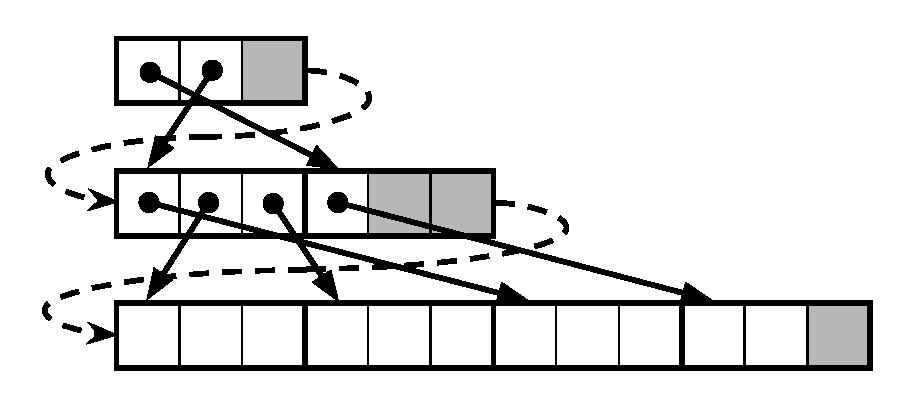
\includegraphics[scale=0.5]{memory_layout}
    \caption{R-tree memory layout with \(r = 3\).}
    \label{fig:memory-layout}
\end{figure}

Each record in the array is a \(\{mbb, score, idx\}\) tuple. For leaf node records, the \(mbb\) and \(score\) fields contain the MBB and score of an entry in the R-tree, while the remaining \(idx\) field is left unused. For inner node records, the \(mbb\) field contains the MBB of the node, and the \(score\) field contains an aggregation of the \(score\) of its children. The \(idx\) field contains the position of the block in the array that contains the records of the node.

Each block has a fixed size of \(r\) records. For a fully packed node, the block is full, but for non-full nodes, the rightmost records are used as padding. In practice, all blocks but the final block of a segment are fully packed. To access the MBBs and score (and child node references) of all the records of a node, all that has to be accessed is one fixed size block which will never be out of bounds for nodes that are not filled to capacity. For a sufficiently large input, the memory used by the padding should be negligible.

The R-tree memory layout is designed for storage in global memory on the GPU. While storing the R-tree in shared memory would allow much faster access, the R-trees are expected to be too large to fit in shared memory. Therefore, special attention is given to the alignment and size of the blocks of the record array. Ideally, blocks should be laid out so that they are naturally aligned with the memory transactions between the L1 cache, L2 cache and global memory. This allows efficiently fetching all records of a node.

\section{GPU aR-tree bulk loading}

A key element of the performance of the Depth-First Algorithm and the Block-based Algorithm is bulk loading. The Block-based algorithm performs a number of small bulk loads, and the Depth-First Algorithm performs two large bulk loads (assuming the R-trees have not been constructed prior to performing the join). To experiment with performing these algorithms on the GPU, we are interested in utilizing the GPU to perform bulk loading.

It is assumed that the unindexed data resides in device memory and that the resulting R-tree data structure will also reside in device memory. If the unindexed data originates from host memory, the unindexed data first has to be transferred to device memory. The bulk loading algorithm operates entirely within device memory, and can be controlled by a program either on the GPU or the CPU.

The bulk-loading algorithm is based on Sort-Tile-Recursive and produces an aR-tree with the aforementioned layout. Using a precomputed segment layout, it allocates an array of R-tree node records and places the data as records in the bottom level segment, then builds the R-tree from the bottom up, segment by segment until it reaches the root. The algorithm is powered by radix sort, which is a sorting algorithm that is highly efficient on the GPU.

\subsection{Computed layout}

Prior to building the R-tree, a segment layout has to be computed based on the size of the input and the fanout of the R-tree. Given an input of size \(n\) and a fanout of \(r\), the Layout Algorithm returns a segmentation of an R-tree array that fits any input of size \(n\), expressed as a list of segment sizes and offsets. The layout is only a function of the size of the input and the fanout of an R-tree that is to be bulk-loaded, it is not dependent on the actual records of the R-tree. Therefore, for repeated bulk loads such as the ones used in the Block-based Algorithm, the segmentation can be memoized and re-used for multiple bulk loads.

\begin{algorithm}
  \caption{Layout Algorithm. \(n\) is the amount of entries in the R-tree, and \(r\) is the fanout of the R-tree.}
  \label{alg/layout}
  \begin{algorithmic}[1]
    \Function{Layout}{\protect\(n, r\protect\)}
      \State{Initialize L as list of \(\lceil log_r(n) \rceil\) elements}
      \State \(i \gets 0\)
      \Repeat
        \State \(n \gets \lceil \frac{n}{r} \rceil\)
        \State \(L_i.\mathrm{size} \gets n \times r\)
        \State \(i \gets i + 1\)
      \Until{\(n \leq 1\)}
      \State \(o \gets 0\)
      \Repeat
        \State \(i \gets i - 1\)
        \State \(L_i.\mathrm{offset} \gets o\)
        \State \(o \gets o + S_i.\mathrm{size}\)
      \Until{\(i = 1\)}
      \State \Return \(L\)
    \EndFunction
  \end{algorithmic}
\end{algorithm}

The intuitive explanation for the Layout Algorithm is that \(n\) R-tree node records must be distributed into at least \(\left\lceil \frac{n}{r} \right\rceil\) nodes of size \(r\). By bulk loading \(n\) R-tree entries, \(n\) leaf node records must be distributed into at least \(\left\lceil \frac{n}{r} \right\rceil\) leaf nodes. Each leaf node will have to be placed as record in an inner node, so the process is repeated for a smaller set of \(\lceil \frac{n}{r} \rceil\) records. When the process encounters \(n \leq r\), the records can only be placed in a single node, which will become the root node.

In the basic case of \(n \leq r\), the R-tree will only be a root, and the algorithm returns the layout of a single segment for the root with a size of \(r\) and an offset of zero. When \(n > r\), the algorithm returns a layout of multiple segments. Each segment must be offset by the cumulative size of the segments of the above levels. Because \(L_1\) will lay out the last segment of the array, the total size of the array can be computed as \(L_1.\mathrm{offset} + \ L_1.\mathrm{size}\).

\subsection{Tile Partition Algorithm}

The Tile Partition Algorithm takes a segment of an R-tree record array \(S\) and partitions the records of \(S\) it into groups of size \(r\) called tiles. The algorithm is used to arrange the node records in a segment of the R-tree record array into blocks with minimal overlap.

\begin{figure}[h]
    \centering
    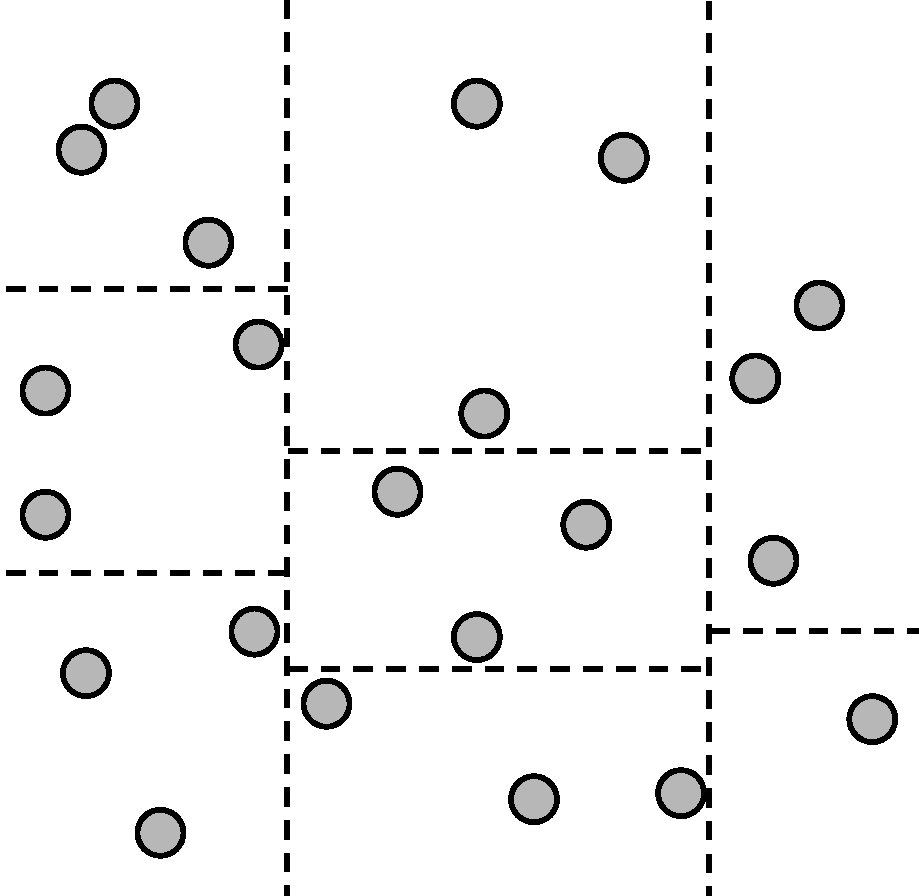
\includegraphics[scale=0.5]{sort_tile_recursive}
    \caption{Tile partitioning of 22 records for \(r = 3\), first sorted by \(x\) coordinate (left to right) then \(y\) coordinate (top to bottom).}
    \label{fig:sort-tile-recursive}
\end{figure}

The algorithm relies on a segmented sorting algorithm. Given an array of keys \(K\), an array of values \(S\) and a segment size of \(s\), the segmented sorting algorithm divides the input into \(k\) segments of size \(s\) \(K_0, K_1, \dotsc, K_{k - 1}\) and \(S_0, S_1, \dotsc, S_{k - 1}\), then sorts each pair \((K_i, S_i)\) independently. The sorting operation sorts the values by their associated keys. Segmented sorting can be parallelized using radix sort on the GPU.

\begin{algorithm}
  \caption{Tile Partition Algorithm. \(S\) is a segment of the R-tree record array, \(r\) is the block size, and \(d\) is the number of dimensions.}
  \label{alg/tile-partition}
  \begin{algorithmic}[1]
    \Function{GpuTilePartition}{\protect\(S, r, d\protect\)}
      \State{Initialize K as list of \(|S|\) elements}
      \State{\(s \gets \left\lceil \sqrt[k]{\frac{|S|}{r}} \right\rceil\)}
      \State{\(l \gets r d^{k}\)}
      \For{\(i \gets 0, d - 1\)}
        \ForAll{\(j \in 0, 1, \dotsc, |S| - 1\) in parallel}
          \State{\(K_j \gets S_j.\mathrm{mbb}.\min_i\)}
        \EndFor
        \State{\(S \gets\) \Call{SegmentedRadixSort}{K, S, l}}
        \State{\(l \gets \frac{s}{s}\)}
      \EndFor
      \State \Return \(S\) 
    \EndFunction
  \end{algorithmic}
\end{algorithm}

The algorithm works by iteratively dividing the input into smaller segments, considering one dimension at a time. In the two-dimensional case, the algorithm first divides the input into vertical slices, then it divides each slice into tiles (blocks). In the three-dimensional case, the algorithm first divides the input into slabs, then divides each slab into pillars, then divides each pillar into a block. \(l\) represents the current size of each segment, and is initially as large as the input segment. \(s\) represents the amount of segments each segment can be divided into, leading to a total of \(s^k\) groups, which has to satisfy the requirement \(r s^k \geq |S|\). If \(|S|\) is not divisible by \(r d^k\), the final segment may contain fewer records than the others.

\subsection{Tile Build Algorithm}

After partitioning of the R-tree node records of a level \(i\), the records of level \(i + 1\) can be produced. The Tile Build Algorithm takes an input segment of R-tree node records and returns an output segment of inner node records. It calculates and records the aggregate score and the MBBs of the inner node records. The score aggregation is MAX, which creates upper bounds.

\begin{algorithm}
  \caption{Tile Build Algorithm. \(S\) is a segment of the R-tree record array and \(r\) is the block size.}
  \label{alg/tile-build}
  \begin{algorithmic}[1]
    \Function{GpuTileBuild}{\protect\(S, r\protect\)}
      \State Initialize \(O\) as list of \(\lceil |S| / r \rceil\) elements
      \ForAll{\(i \in 0, 1, \dotsc, \lceil |S| / r \rceil - 1\) in parallel}
        \State{\(j \gets ir\)}
        \State{\(k \gets\) \Call{Min}{\protect\(j + r, |S|\protect\)}}
        \State{\(O_i.\mathrm{mbb} \gets\) \Call{Reduce}{Mbb, \protect\(\{S_j.\mathrm{mbb}, S_{j + 1}.\mathrm{mbb}, \dotsc, S_{k - 1}.\mathrm{mbb} \}\protect\)}}
        \State{\(O_i.\mathrm{score} \gets\) \Call{Reduce}{MAX, \protect\(\{S_j.\mathrm{score}, S_{j + 1}.\mathrm{score}, \dotsc, S_{k - 1}.\mathrm{score}\}\protect\)}}
        \State{\(O_i.\mathrm{idx} \gets j\)}
      \EndFor
      \State \Return \(O\)
    \EndFunction
  \end{algorithmic}
\end{algorithm}

A key detail is that the Tile Build Algorithm is not limited to parallelization per output element. In fact, it can be efficiently parallelized with a thread per input element. On GPU, the evaluation of each MBB and score MAX value in the output can be evaluated using parallel reduce operations.

\subsection{STR}

Finally, the full Sort-Tile-Recursive algorithm can be described in full. Given an input \(I\) of \(n\) elements, each with a score and an MBB, it returns an array of R-tree records according to the layout \(L\) that contains the input elements. First, the STR algorithm places the input data as leaf node records in the final segment of the array of R-tree records. Then for all but the last level (the root level), the algorithm first partitions the node records of the current level into tiles, then builds the next level of node records. The last level is guaranteed to consist of only the root node and is of size \(r\), therefore it requires no sorting, nor has any level above it to be built. The resulting array contains all segments in descending order of level.

\begin{algorithm}
  \caption{STR. \(L\) is the layout of the R-tree, \(I\) is a list of entries to be inserted, \(r\) is the block size and \(d\) is the number of dimensions.}
  \label{alg/str}
  \begin{algorithmic}[1]
    \Function{GpuStr}{\protect\(L, I, r, d\protect\)}
      \State Initialize \(R\) as list of \(L_0.\mathrm{offset} + L_0.\mathrm{size}\) elements
      %\State Initialize \(S\) as list of \(h\) elements
      \ForAll{\(i \in 0, 1, \dotsc, n - 1\) in parallel}
        \State \(R_{L_0.\mathrm{offset} + i}.\mathrm{mbb} = I_i.\mathrm{mbb}\)
        \State \(R_{L_0.\mathrm{offset} + i}.\mathrm{score} = I_i.\mathrm{score}\)
      \EndFor
      \For{\(i \gets 0,\, |L| - 1\)}
        \State \(j_0 \gets L_i.\mathrm{offset}\)
        \State \(k_0 \gets j_0 + L_i.\mathrm{size} - 1\)
        \State \(j_1 \gets L_{i + 1}.\mathrm{offset}\)
        \State \(k_1 \gets j_1 + L_{i + 1}.\mathrm{size} - 1\)
        \State \(R_{j_0, j_0 + 1, \dotsc, k_0} \gets\) \Call{GpuTilePartition}{\protect\(R_{j_0, j_0 + 1, \dotsc, k_0}, r, d\protect\)}
        \State \(R_{j_1, j_1 + 1, \dotsc, k_1} \gets\) \Call{GpuTileBuild}{\protect\(R_{j_0, j_0 + 1, \dotsc, k_0}, r\protect\)}
      \EndFor
      \State \Return \(R\)
    \EndFunction
  \end{algorithmic}
\end{algorithm}

\section{GPU top-k R-tree join}

The GPU Ranked R-tree Join Algorithm is based on the work of Qi et al.~\cite{qi2013efficient}. Given two aR-trees \(A\) and \(B\), it returns the top-\(k\) joined elements above the score threshold \(\theta\). The threshold may be set to \(\theta = -\infty\), in which case the threshold is effectively ignored. The algorithm is a key part of both the Distance-First Algorithm and the Block-based Algorithm.

The algorithm operates on a priority queue implemented as a parallel heap that resides. Each element in the queue refers to two intersecting nodes, one from \(A\) and the other from \(B\). The priority queue is initialized with references to the root nodes of \(A\) and \(B\). In each pass, the top element of the queue is dequeued, then all records of the node of \(A\) and \(B\) are fetched from global memory. Then all combinations of node records are evaluated in parallel, producing anywhere from zero to \(r^2\) results which are temporarily placed into \(V\) as candidate result. \(V\) may contain a number of \(Nil\) values, so \(V\) is compacted to filter out \(Nil\) entries. If the records are inner node records, the elements of \(V\) are placed into the priority queue. If not, the elements of \(V\) are placed as candidate results into \(C\) so that \(C\) retains the current top-\(k\) elements.

The score threshold \(\theta\) is continuously updated to represent the \(k^{th}\) greatest score seen so far when candidate results are discovered. Until \(k\) candidate results are discovered, \(\theta\) remains at its initial value. When an element of the priority queue is dequeued with a score below \(\theta\), the join can no longer produce elements with a score that satisfies the score threshold, so the algorithm terminates. The algorithm will also terminate if the queue has no remaining elements.

\begin{algorithm}
  \caption{Ranked R-tree Join Algorithm. \(k\) is the amount of elements to be returned, \(A\) is the first R-tree, \(B\) is the second R-tree, \(\theta\) is the score threshold, \(\phi\) is the spatial predicate used to join the R-tree nodes and \(\gamma\) is the score aggregate function.}
  \label{alg/ranked-r-tree-join}
  \begin{algorithmic}[1]
    \Function{GpuRankedRTreeJoin}{\protect\(k, A, B, \theta, \gamma, \phi\protect\)}
      \State Initialize \(Q\) as a priority queue with initial entry \(\{ .score=0,\, .level=h - 1,\, .aIdx=0,\, .bIdx=0 \}\)
      \State Initialize \(C\) as shared list of size \(k\)
      % \State Initialize \(T\) and \(U\) as shared lists of size \(r\)
      \State Initialize \(V\) as a shared list of size \(r^2\)
      \While{\(Q\) is not empty}
        \State \(e \gets\) \Call{Dequeue}{\protect\(Q\protect\)}
        \If{\(e.\mathrm{score} < \theta\)}
          \State \Return \(C\) \Comment{No more elements with sufficient score}
        \EndIf
        % \ForAll{\(i \in 0, 1, \dotsc, r - 1\) in parallel}
        %   \State \(T_i \gets A_{e.\mathrm{aIdx} + i}\)
        %   \State \(U_i \gets B_{e.\mathrm{bIdx} + i}\)
        % \EndFor
        \ForAll{\((i, j) \in (0, 1, \dotsc, r - 1) \times (0, 1 \dotsc, r- 1)\) in parallel}
          \State \(s \gets\) \Call{\(\gamma\)}{\protect\(A_{e.\mathrm{aIdx} + i}.\mathrm{score}, B_{e.\mathrm{bIdx} + j}.\mathrm{score}\protect\)}
          \If{\Call{\(\phi\)}{\protect\(A_{e.\mathrm{aIdx} + i}.\mathrm{mbb}, B_{e.\mathrm{bIdx} + j}.\mathrm{mbb}\protect\)} and \(s \geq \theta\)}
            \State \(V_{rj + i}.\mathrm{score} \gets s\)
            \State \(V_{rj + i}.\mathrm{level} \gets e.\mathrm{level} - 1\)
            \State \(V_{rj + i}.\mathrm{aIdx} \gets A_{e.\mathrm{aIdx} + i}.\mathrm{idx}\)
            \State \(V_{rj + i}.\mathrm{bIdx} \gets B_{e.\mathrm{bIdx} + j}.\mathrm{idx}\)
          \Else
            \State \(V_{rj + i} \gets Nil\)
          \EndIf
        \EndFor
        \State \Call{Compact}{\protect\(V\protect\)}
        \If{\(e.\mathrm{level} > 0\)} \Comment{Pairs of inner node records}
          \State \Call{Enqueue}{\protect\(Q, V\protect\)}
        \Else \Comment{Pairs of leaf node records}
          \State \(C \gets\) \Call{TopK}{\protect\(C + V, k\protect\)}
          \If{\(|C| = k\)}
            \State \(\theta \gets C_{k - 1}\)
          \EndIf
        \EndIf
      \EndWhile
      \State \Return \(C\) \Comment{No more elements}
    \EndFunction
  \end{algorithmic}
\end{algorithm}

The main draw of the algorithm is that it is an implementation of a ranked R-tree join that can run on the GPU, but its performance is expected to be limited. Even though the algorithm can utilize parallelism to evaluate the spatial predicate for all combinations in parallel on the GPU, it is not expected to outperform an implementation of a ranked R-tree join on the CPU in the general case. The reason for this is that the cost of compacting, sorting and maintaining the priority queue is expected to be high. Additionally, the kernel will be spending some time waiting for the node records to be fetched from global memory. The algorithm can instead be parallelized by running multiple instances of the algorithm in parallel. The algorithm fits naturally into a thread group of size \(r^2\), so a number of thread groups can be created to allow interleaved execution multiple ranked R-tree joins.

Ideally, the parallel heap will reside in shared memory for its fast memory access characteristics, but shared memory may not be able to hold enough elements for sufficiently large values of \(k\) or large R-trees with bad score distributions. Even if the queue is small enough to fit into shared memory, it should also be sufficiently small to allow multiple thread blocks to execute on the same streaming multiprocessor. The top of the parallel heap could be placed in shared memory and the while could be placed in global memory. Alternatively, when the queue grows sufficiently large, the task could be divided into subproblems by distributing the elements of the parallel heap into additional thread groups, then concatenating their top-k results. Another strategy would be to keep the size of the R-trees sufficiently small to prevent overflow.

\section{GPU Block-based Algorithm}

Like the Block-based Algorithm, the GPU Block-based Algorithm reads the inputs in order of descending rank, one block at a time. It uses the GPU STR algorithm to bulk load R-trees from each loaded input block, then evaluates a GPU ranked R-tree join in parallel for each previously loaded block of the other input. Similar to HRJN, the aggregate score of the last accessed item of input A and the first accessed item of input B forms an upper bound for the score of any joined item produced by reading another block of A, and the aggregate score of the last accessed item of input B and the first accessed item of input A forms an upper bound for the score of any joined item produced by reading another block of B. This is used to create a threshold \(T\) for all join results that have not been produced. When the \(k^{th}\) candidate result has a score above the threshold, the candidate results of \(C\) are known to be the top-k result.

Assuming the inputs reside in host memory, the inputs have to be transferred to device memory first. Before joining, the unindexed inputs have to be sorted in descending order of score. If they are not already sorted, the sort can be performed entirely on the GPU using radix sort.

The algorithm is expected to start relatively slow due to a limited level of parallelism, but its parallelism scales as more blocks are read and bulk loaded into R-trees. Each time a block is read and bulk loaded into an R-tree, another join can be performed in parallel. The rate of increase in parallelism is dependent to the block size, which should be kept relatively low for sufficient increase in parallelism, though increasing levels of parallelism will increase the amount of work.

\begin{algorithm}
  \caption{Block-based Algorithm. \(k\) is the amount of elements to return, \(A\) and \(B\) are the spatial inputs, \(\gamma\) is the score aggregate function and \(\phi\) is the spatial predicate.}
  \label{alg/block-based}
  \begin{algorithmic}[1]
    \Function{GpuBlockTopK}{\protect\(k, A, B, \gamma, \phi\protect\)}
      \State Initialize \(C\) as list of size \(k\)
      \State Sort \(A\) and \(B\) if not already sorted
      \State \(\theta \gets -\infty\)
      \While{more blocks of objects exist in \(A\) and \(B\)}
        \State \(i \gets\) next input to be accessed \Comment{\(A\) or \(B\)}
        \State \(j \gets\) the other input \Comment{\(A\) or \(B\)}
        \State \(P \gets\) \Call{GetNextBlock}{\protect\(i\protect\)}
        \State \(L \gets\) \Call{Layout}{\protect\(|P|, r\protect\)}
        \State \(R_P \gets\) \Call{GpuStr}{\protect\(L, P, r, \gamma_l, k\protect\)}
        \State Initialize \(V\) as list
        \ForAll{blocks \(P'\) of \(j\) in parallel}
          \State \(V \gets V +\) \Call{GpuRankedRTreeJoin}{\protect\(k, R_P, {R_P}', \theta, \gamma_r, \phi\protect\)}
        \EndFor
        \State \(C \gets\) \Call{TopK}{\protect\(k, C + V\protect\)}
        \If{\(|C| = k\)}
          \State \(\theta \gets C_{k - 1}\)
        \EndIf
        \State \(T \gets \mathrm{MAX}(\gamma(A_{first}.\mathrm{score}, B_{last}.\mathrm{score}), \gamma(A_{last}.\mathrm{score}, B_{first}.\mathrm{score}))\)
        \If{\(T < \theta\)}
          \State \Return \(C\) \Comment{No more elements with sufficient score}
        \EndIf
      \EndWhile
      \State \Return \(C\) \Comment{No more input elements}
    \EndFunction
  \end{algorithmic}
\end{algorithm}


\chapter{Conclusions and future work}
\section{Conclusions}

All parts of the top-k spatial join can be performed on the GPU with varying degrees of parallelism. Efficient utilization of GPGPU can be achieved by identifying the parts of an application that can be parallelized, then finding parallel solutions with respect to GPU architecture, which is significantly different from ordinary processor architecture. The best performance is achieved with special care for memory access and by dividing problems into as many independent tasks as possible that can be executed in parallel.

R-trees can be represented in device memory as a compact array of R-tree node records divided into segments. By placing node records into blocks that are aligned with the memory transactions of the GPU, the cost of random access to all records of a node should be kept as low as possible. They can be efficiently bulk loaded using a series of segmented parallel radix sorts to partition the data into tiles, then using parallel reductions to calculate node MBBs and aggregate data values.

The Block-based Algorithm can be performed entirely on the GPU with all data completely residing within GPU memory. Unindexed inputs can be sorted by score on the GPU using parallel radix sort prior to performing top-k spatial joins. A top-k spatial join can be evaluated in parallel by dividing the problem into multiple top-k spatial joins then finding the top-k elements among the results. Multiple ranked spatial joins on R-trees can be performed in parallel. Moreover, a ranked spatial join on R-trees exhibits parallelism in the form of parallel evaluation of spatial predicates for all combinations of node records. However, the cost of maintaining priority queues is expected to be comparatively high on the GPU.

While most of the methods presented are based on proven GPGPU methods that have exhibited speedups, the full solution for top-k spatial joins on GPU has not yet been verified by experimentation. There may be unknown factors affecting the performance, and a number of tweaks may be necessary to achieve competitive performance. However, crafting a parallelized version of an existing algorithm is a necessary first step in achieving top-k spatial joins on GPU.

\section{Future work}

An necessary continuation of this work is an evaluation of the methods presented by implementing them in CUDA and experimenting with various data of different distributions and sizes. A natural comparison would be between single-threaded implementations, multi-threaded implementations and GPGPU implementations. While the original Block-based algorithm has been tested and proven to be efficient, the adaptation for GPGPU may not be as efficient due to a number of unknown factors or challenges in the implementation. The only way to verify the viability of these methods is by experimentation and iterating on the solution based on performance analysis.

An interesting modification could be modifying the R-tree memory layout so that the R-tree node records are stored in breadth-first order. The reason that this is an interesting modification is because it would render the \(idx\) field of the inner node records obsolete. If an inner node record is stored at position \(i\) of a segment of an R-tree record array, then the records of the node are stored in the \(i^{th}\) block in the next segment. By removing the \(idx\) field, the required size of each record in memory is reduced, which may relax the padding requirements. By reducing the size of the R-tree in memory, less memory bandwidth would be required which would increase the performance. However, this would require a different bulk loading implementation that can produce R-trees in breadth-first order.

Another avenue of research for top-k spatial joins is using other data structures such as the family of quadtree data structures. The R-tree is considered a data-driven spatial data structure because the way it partitions the space is dependent on the data. Unlike the R-tree, the quadtree is considered a space-driven spatial data structure because it uses a fixed division of the space. Because the division of the space is not dependent on the data, quadtree bulk loading methods may be able to more efficiently partition the data. However, for data whose indexed spatial attributes cannot be represented as a single point, duplicate entries may have to be inserted into the quadtree, which introduces the problem of eliminating duplicates during spatial joins which would present some challenges, especially for parallel evaluation of top-k queries.

Another surprisingly simple way to achieve parallel top-k spatial joins might be using a parallel plane-sweep based join. While the plane sweep join algorithm cannot produce outputs in ranked order, a number of top-k joins could be performed in parallel by sorting then dividing the data into different segments and performing a top-k join on each segment. The top-k results could then be joined into a single top-k result.


%\appendix
%\chapter{Example appendix}
%\input{chapters/appendix}

\printbibliography{}

\end{document}
